\documentclass[class=minimal,border=10pt]{standalone}
\usepackage{makecell}
\usepackage{tikz}
\usetikzlibrary{positioning}
\begin{document}
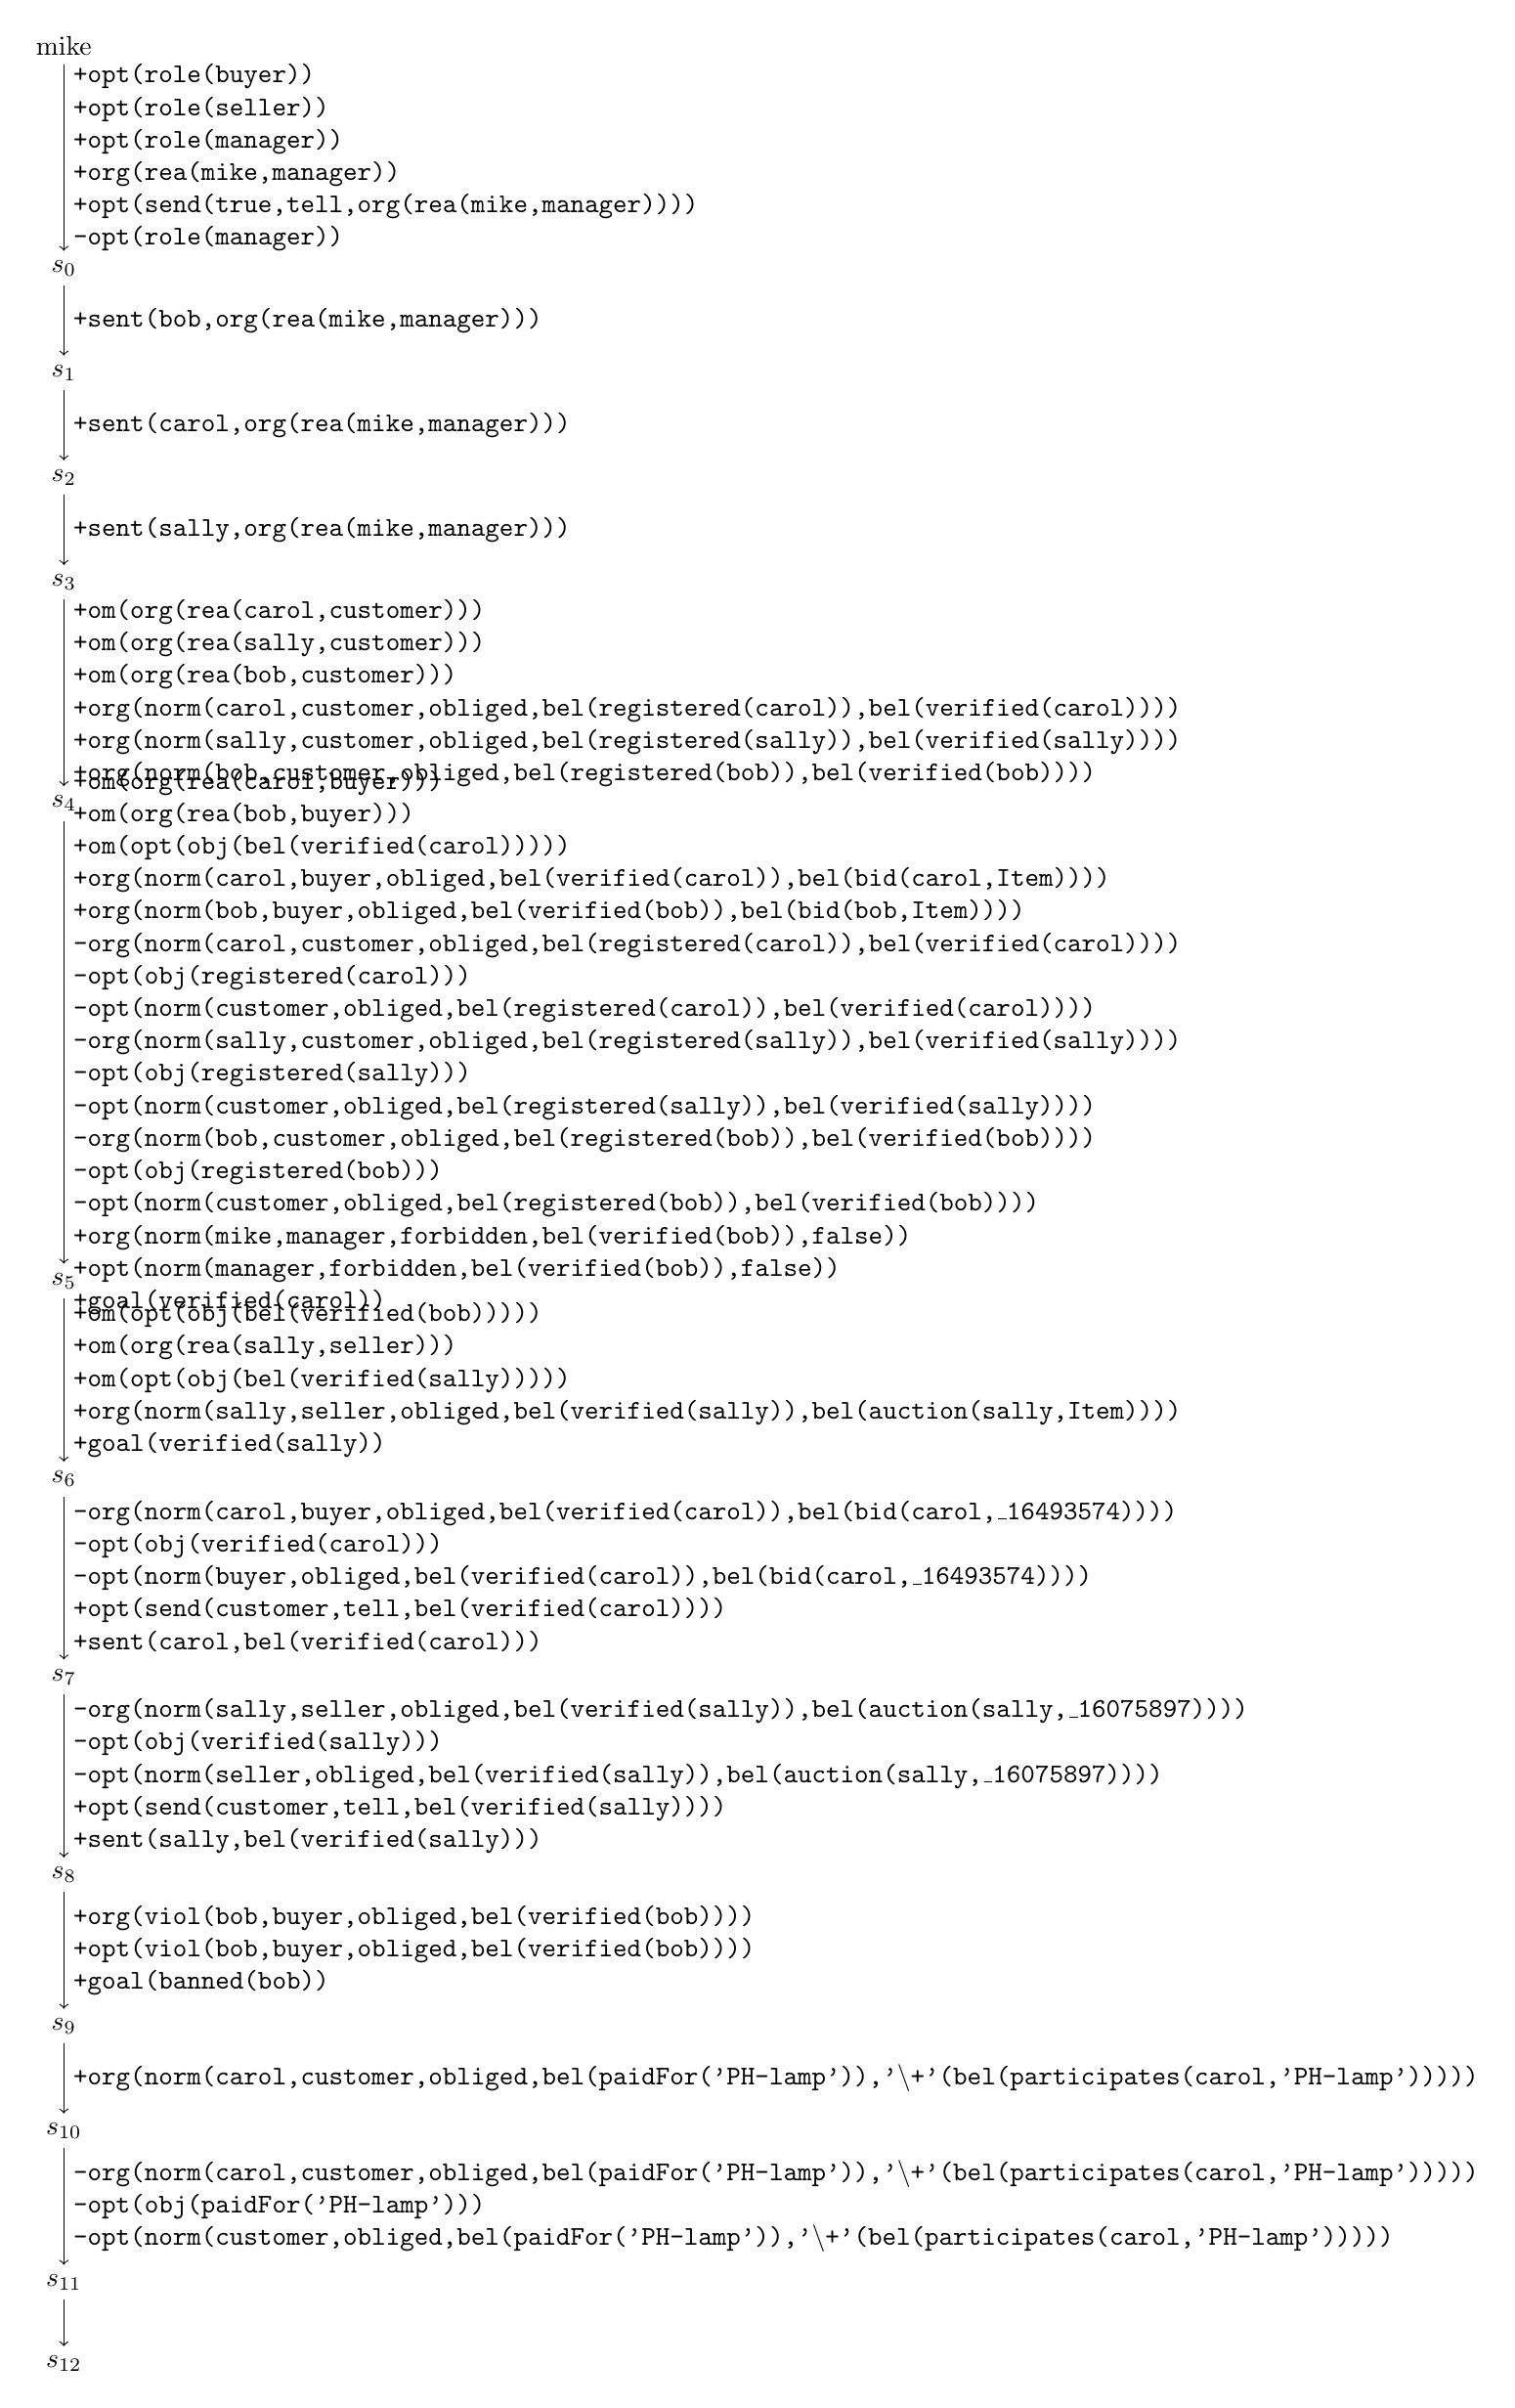
\begin{tikzpicture}[->]
\tikzstyle{node} = [font=\normalfont]\node[node] (agent) {mike};
\node[node, below=16ex of agent] (s0) {$s_{0}$};
\draw (agent) -- node[auto=left] {\makecell[l]{
\texttt{+opt(role(buyer))}\\
\texttt{+opt(role(seller))}\\
\texttt{+opt(role(manager))}\\
\texttt{+org(rea(mike,manager))}\\
\texttt{+opt(send(true,tell,org(rea(mike,manager))))}\\
\texttt{-opt(role(manager))}\\
}} (s0);
\node[node, below=6ex of s0] (s1) {$s_{1}$};
\draw (s0) -- node[auto=left] {\makecell[l]{
\texttt{+sent(bob,org(rea(mike,manager)))}\\
}} (s1);
\node[node, below=6ex of s1] (s2) {$s_{2}$};
\draw (s1) -- node[auto=left] {\makecell[l]{
\texttt{+sent(carol,org(rea(mike,manager)))}\\
}} (s2);
\node[node, below=6ex of s2] (s3) {$s_{3}$};
\draw (s2) -- node[auto=left] {\makecell[l]{
\texttt{+sent(sally,org(rea(mike,manager)))}\\
}} (s3);
\node[node, below=16ex of s3] (s4) {$s_{4}$};
\draw (s3) -- node[auto=left] {\makecell[l]{
\texttt{+om(org(rea(carol,customer)))}\\
\texttt{+om(org(rea(sally,customer)))}\\
\texttt{+om(org(rea(bob,customer)))}\\
\texttt{+org(norm(carol,customer,obliged,bel(registered(carol)),bel(verified(carol))))}\\
\texttt{+org(norm(sally,customer,obliged,bel(registered(sally)),bel(verified(sally))))}\\
\texttt{+org(norm(bob,customer,obliged,bel(registered(bob)),bel(verified(bob))))}\\
}} (s4);
\node[node, below=38ex of s4] (s5) {$s_{5}$};
\draw (s4) -- node[auto=left] {\makecell[l]{
\texttt{+om(org(rea(carol,buyer)))}\\
\texttt{+om(org(rea(bob,buyer)))}\\
\texttt{+om(opt(obj(bel(verified(carol)))))}\\
\texttt{+org(norm(carol,buyer,obliged,bel(verified(carol)),bel(bid(carol,Item))))}\\
\texttt{+org(norm(bob,buyer,obliged,bel(verified(bob)),bel(bid(bob,Item))))}\\
\texttt{-org(norm(carol,customer,obliged,bel(registered(carol)),bel(verified(carol))))}\\
\texttt{-opt(obj(registered(carol)))}\\
\texttt{-opt(norm(customer,obliged,bel(registered(carol)),bel(verified(carol))))}\\
\texttt{-org(norm(sally,customer,obliged,bel(registered(sally)),bel(verified(sally))))}\\
\texttt{-opt(obj(registered(sally)))}\\
\texttt{-opt(norm(customer,obliged,bel(registered(sally)),bel(verified(sally))))}\\
\texttt{-org(norm(bob,customer,obliged,bel(registered(bob)),bel(verified(bob))))}\\
\texttt{-opt(obj(registered(bob)))}\\
\texttt{-opt(norm(customer,obliged,bel(registered(bob)),bel(verified(bob))))}\\
\texttt{+org(norm(mike,manager,forbidden,bel(verified(bob)),false))}\\
\texttt{+opt(norm(manager,forbidden,bel(verified(bob)),false))}\\
\texttt{+goal(verified(carol))}\\
}} (s5);
\node[node, below=14ex of s5] (s6) {$s_{6}$};
\draw (s5) -- node[auto=left] {\makecell[l]{
\texttt{+om(opt(obj(bel(verified(bob)))))}\\
\texttt{+om(org(rea(sally,seller)))}\\
\texttt{+om(opt(obj(bel(verified(sally)))))}\\
\texttt{+org(norm(sally,seller,obliged,bel(verified(sally)),bel(auction(sally,Item))))}\\
\texttt{+goal(verified(sally))}\\
}} (s6);
\node[node, below=14ex of s6] (s7) {$s_{7}$};
\draw (s6) -- node[auto=left] {\makecell[l]{
\texttt{-org(norm(carol,buyer,obliged,bel(verified(carol)),bel(bid(carol,\_16493574))))}\\
\texttt{-opt(obj(verified(carol)))}\\
\texttt{-opt(norm(buyer,obliged,bel(verified(carol)),bel(bid(carol,\_16493574))))}\\
\texttt{+opt(send(customer,tell,bel(verified(carol))))}\\
\texttt{+sent(carol,bel(verified(carol)))}\\
}} (s7);
\node[node, below=14ex of s7] (s8) {$s_{8}$};
\draw (s7) -- node[auto=left] {\makecell[l]{
\texttt{-org(norm(sally,seller,obliged,bel(verified(sally)),bel(auction(sally,\_16075897))))}\\
\texttt{-opt(obj(verified(sally)))}\\
\texttt{-opt(norm(seller,obliged,bel(verified(sally)),bel(auction(sally,\_16075897))))}\\
\texttt{+opt(send(customer,tell,bel(verified(sally))))}\\
\texttt{+sent(sally,bel(verified(sally)))}\\
}} (s8);
\node[node, below=10ex of s8] (s9) {$s_{9}$};
\draw (s8) -- node[auto=left] {\makecell[l]{
\texttt{+org(viol(bob,buyer,obliged,bel(verified(bob))))}\\
\texttt{+opt(viol(bob,buyer,obliged,bel(verified(bob))))}\\
\texttt{+goal(banned(bob))}\\
}} (s9);
\node[node, below=6ex of s9] (s10) {$s_{10}$};
\draw (s9) -- node[auto=left] {\makecell[l]{
\texttt{+org(norm(carol,customer,obliged,bel(paidFor('PH-lamp')),'\textbackslash{+}'(bel(participates(carol,'PH-lamp')))))}\\
}} (s10);
\node[node, below=10ex of s10] (s11) {$s_{11}$};
\draw (s10) -- node[auto=left] {\makecell[l]{
\texttt{-org(norm(carol,customer,obliged,bel(paidFor('PH-lamp')),'\textbackslash{+}'(bel(participates(carol,'PH-lamp')))))}\\
\texttt{-opt(obj(paidFor('PH-lamp')))}\\
\texttt{-opt(norm(customer,obliged,bel(paidFor('PH-lamp')),'\textbackslash{+}'(bel(participates(carol,'PH-lamp')))))}\\
}} (s11);
\node[node, below=4ex of s11] (s12) {$s_{12}$};
\draw (s11) -- node[auto=left] {\makecell[l]{
}} (s12);
	\end{tikzpicture}
\end{document}